\chapter{Hadronic recoil regression with deep neural networks}

In the recent years a significant progress was achieved in the field of big datasets analysis. There is a number of principles available for solving a wide variety of tasks. In this thesis a \gls{dnn} was used for the regression of the 2-component hadronic recoil vector.
\section{Deep neural networks}
Normally a machine learning problem has a number of ingredients: a dataset \textbf{X}, a set of parameters \textbf{$\theta$}, a model  $g(\theta)$ and a loss function $C(\textbf{X})$ that tells us how well the model $g(\textbf{\theta})$ describes the dataset. Finding the values of \textbf{$\theta$} that would minimize the loss function we fit the model.
\subsection{Gradient descent optimization}
One of the most powerful and used class of methods in minimizing the loss function is called the \textit{gradient descent}, \cite{gradient} especially its sub-class, the \gls{sgd} \cite{sgd1}, \cite{sgd2}. One of its modifications called ADAM \cite{kingma2014method} was used as an optimization algorithm in the work presented in this thesis. \\
Let's assume that a loss function $E(\theta)$ may be estimated as a sum over n data points:
\begin{equation}
E(\theta) = \sum^n_{i=1} e_i(x_i,\theta).
\end{equation}
In the simplest case of the \gls{gd} algorithm we start looking for the values of parameters $\theta$ such that the sum of functions $\sum^n_{i=1}e_i$ is minimal. We start with a certain value $\theta_0$ and then iteratively perform the following:
\begin{equation}
\begin{array}{lcl} 
v_t=\eta_t\nabla_{\theta}E(\theta_t),\\
\theta_{t+1}=\theta_t-v_t,
\end{array} 
\end{equation}
where $\nabla_{\theta}E(\theta_t)$ is the gradient of $E(\theta)$ with respect to $\theta$; factor $\eta_t$ is called the \textit{learning rate} and defines the length of the step in the direction of $\theta$ performed with every iteration. Balancing learning rate is very important for learning process and convergence. A value too low can make the convergence "stuck" in the local minimum, it also increases the number of iterations. Picking a very high learning rate we risk to miss the minimum so the algorithm would never converge to a minimum. Also, if the number of data points $n$ is high, calculating the gradient is a costly task in terms of CPU time. \\
Some of the problems accompanying the use of \gls{gd} are dealt with by using its modification - the \gls{sgd}. The idea is the following: instead of using all the available data points $n$ at each iteration of the \gls{gd}, we split the data into $k$ \textit{minibatches}, each having $M$ data points, such that $k = n/M$. Normally the size of the batch is ~few hundreds of data points, to provide a certain degree of variance and incorporating stochasticity. The transition to \gls{sgd} algorithm is done in the following way:
\begin{equation}
\nabla_{\theta}E(\theta) = \sum^n_{i=1} \nabla_{\theta}e_i(x_i,\theta) \rightarrow \sum_{i \in B_l} \nabla_{\theta}e_i(x_i,\theta),
\end{equation}
where $B_l$ is a set of data points belonging to a minibatch $l \in 1, ... , n/M$. Now every next iteration of $\theta$ parameters update is performed over a different batch, consecutively running over all the batches: 
\begin{equation}
\begin{array}{lcl} 
\nabla_{\theta}E^{EM}(\theta) = \sum_{i \in B_l} \nabla_{\theta}e_i(x_i,\theta),\\
v_t=\eta_t\nabla_{\theta}E^{EM}(\theta_t),\\
\theta_{t+1}=\theta_t-v_t.
\end{array} 
\end{equation}
A full iteration over all the $n/M$ batches is called an \textit{epoch}. Now stochasticity prevents the gradient algorithm from getting stuck in a local minimum. Also computing the gradient over fewer data point notably decreases the CPU time spent. \\
The algorithm may be further improved, adding a "memory", that is to say making every next step $t$ dependent on the direction of the previous step $t-1$:
\begin{equation}
\begin{array}{lcl} 
v_t=\gamma v_{t-1}\eta_t\nabla_{\theta}E^{EM}(\theta_t),\\
\theta_{t+1}=\theta_t-v_t.
\end{array} 
\end{equation}
Thanks to analogy from physics the parameter $\gamma$ is called a \textit{momentum}, having $0\le\gamma \le 1$ \cite{grad_momentum1}, \cite{grad_momentum2}. This parameter provides a certain "inertia" in the change of the direction of the gradient descent. Introduction of the momentum helps for quicker convergence in the case of a slow but steady change of a certain parameter during the gradient descent.\\
The convergence of the \gls{gd} may be significantly improved if the learning rate could be different in different directions, depending on the landscape of the parameter space $\theta$: the steeper the gradient in a certain direction - the smaller the corresponding step. The optimal step could be estimated by obtaining the \textit{Hessian matrix} in the vicinity of a point $\theta_0$, providing a description of the local curvature in a multidimensional space. Although calculating Hessian matrix is complicated and slow-converging process \cite{LeCun1998}. However, a number of methods use the second moment of the gradient to efficiently estimate the optimal learning rate. One of such methods is called ADAM (ADAptive Momentum) \cite{kingma2014method}, its iterative relations are the following:
\begin{equation}
\begin{array}{lcl} 
g_t=\nabla_{\theta}E(\theta_t)\\
m_t=\beta_1 m_{t-1}+(1-\beta_1)g_t\\
s_t=\beta_2 s_{t-1} + (1-\beta_2)g_t^2\\
\hat{m_t}=\frac{m_t}{1-(\beta_1)^t}\\
\hat{s_t}=\frac{s_t}{1-(\beta_2)^t}\\
\theta_{t+1}=\theta_t-\eta_t\frac{\hat{m_t}}{\sqrt{\hat{s_t}}+\epsilon}.
\end{array} 
\end{equation}
Here the parameters $\beta_1$ and $\beta_2$ set the memory lifetime for the first and second moment; \eta is the learning rate and $\epsilon$ is a small regularization constant keeping the denominators from vanishing. Like in other cases of the \gls{sgd} here the iterations are performed batch-wise. Parameter $s_t$ is linked to the variance of the gradient size. This basically means that the learning rate is proportional to the first momentum of the gradient and inverse proportional to its standard deviation.
\subsection{DNN structure and training}
A neural network is composed of single neurons, also called nodes, arranged in layers. The first layer is called the input layer, the last one is called the output layer; all the layers in between are named hidden layers (see Fig. \ref{fig::dnn}). \\
A single node $i$ takes a vector of k input features $\textbf{x}=(x_1,x_2,...,x_k)$ and produces a scalar input $a_i(\textbf{x})$. Function $a_i$ may have a different form, although it normally can be decomposed into two steps. The first step is a linear transformation of the inputs into a scalar value assigning each input a weight:
\begin{equation}
z^{i}=w^{i}_k\cdot x_k+b^{i},
\end{equation}
where $\textbf{w}^i=(w^i_1,w^i_2,...,w^i_k)$ is a set of $k$ weights assigned to corresponding inputs. The weights $\textbf{w}^i$ are specific to a neuron $i$, as well as the scalar bias $b^i$. The next step is where the non-linear function $\sigma_i$ comes into play: we can express the output function $a_i(\textbf{x})$ as follows:
\begin{equation}
a_i(\textbf{x})=\sigma_i(z^{i}).
\end{equation}
There exists a number of options for the non-linear function $\sigma$; in current thesis a $\tanh$ is used. When the neurons are arranged in layers in a feed-forward neural network - the outputs from neurons of the previous layer serve as inputs for the succeeding layers neurons. The universal approximation theorem states, that a neural network with a single hidden layer can approximate any continuous multiparametric function with arbitrary accuracy \cite{Kurt1991251}, \cite{Cybenko1989}. However, in practice it is easier to reach the possible precision having more hidden layers. \\
So in terms of a \gls{dnn} fitting the model means tuning the weights and biases $(\textbf{w}^i,b^i)$ in such a way that a loss function applied to the new dataset would be minimal. It is reached through iterative process called \textit{training}, that involves the \gls{gd} with an algorithm called \textit{backpropagation} \cite{RumelhartZipser:86}. The backpropagation algorithm allows to calculate the gradients and adjust the corresponding parameters in a very computation-efficient way. \\
\begin{figure}[htpb]
	\centering
	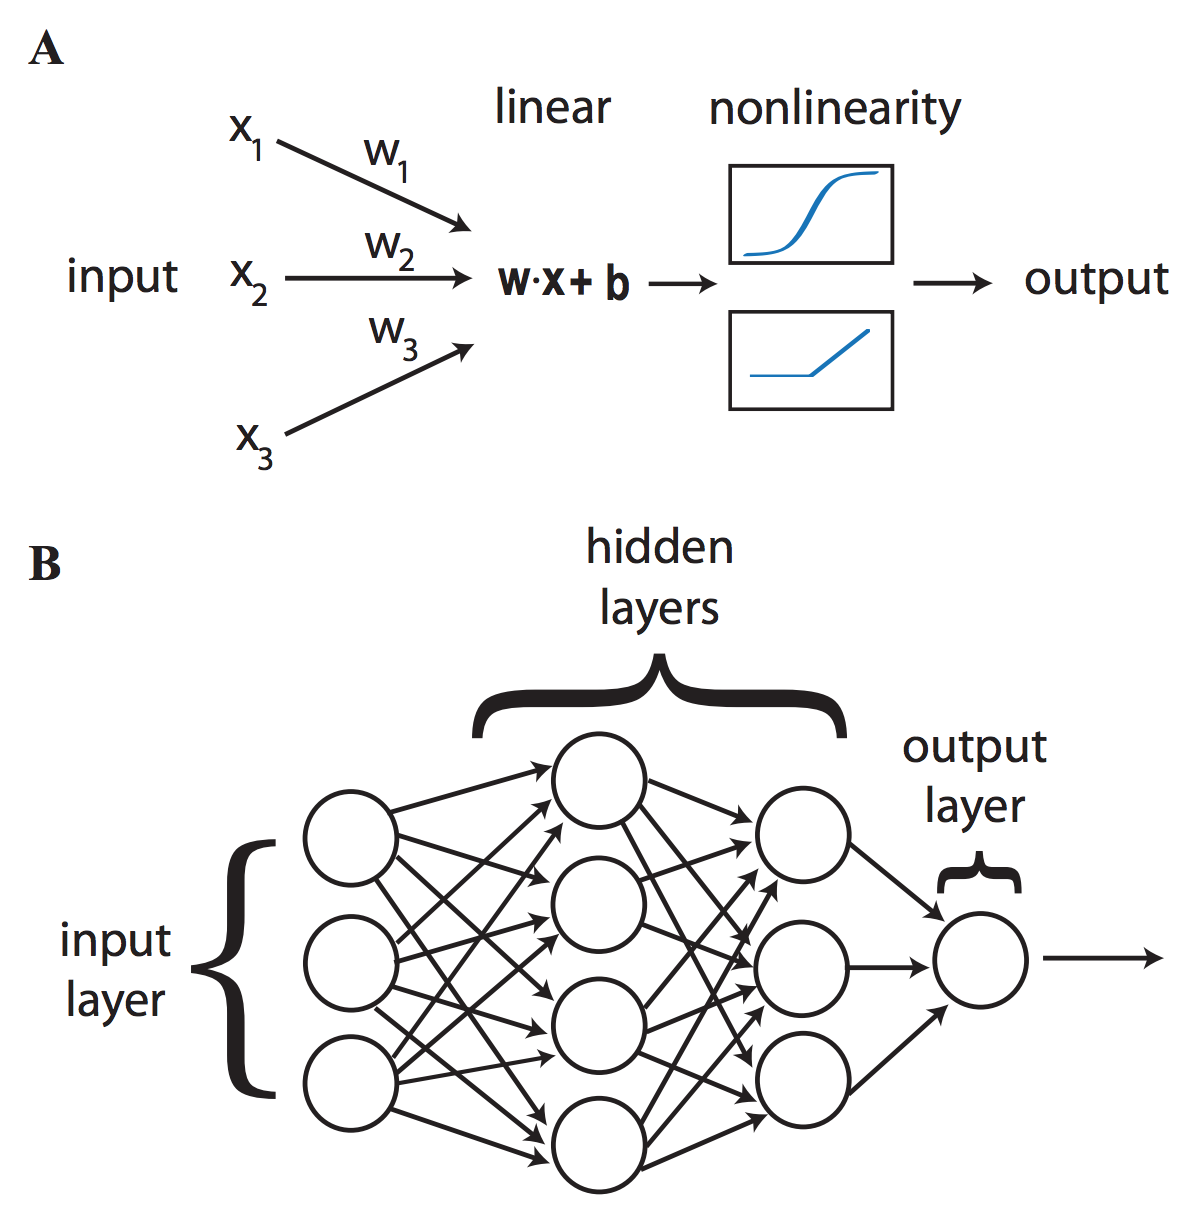
\includegraphics[width=0.5\textwidth,keepaspectratio]{dnn.png}
	\caption{A: The nodes perform a linear transformation of the inputs, then apply a non-linear activation function. B: The architecture of a deep neural network: neurons are arranged into layers~\cite{dnn1}. }
	\label{fig::dnn}
\end{figure}
Let us assume that there are L layers in the network $l=1,...,L$, that $w^l_{jk}$ and $b^l_j$ are the weight of an input parameter k and the bias for node $k$ in layer l respectively. The layered structure of the neural network ensures that the inputs for the nodes in layer $l$ depend only on the outputs of the nodes from layer $l-1$, hence:
\begin{equation}
\label{eq::layer_dep}
a^l_j=\sigma\left(\sum_k w^l_{jk}a^{l-1}_k + b_j^l \right) = \sigma(z^l_j),
\end{equation}
where the linear weighted sum is denoted as:
\begin{equation}
\sigma(z^l_j)=\sum_k w^l_{jk}a^{l-1}_k + b_j^l.
\end{equation}
The cost function E is computed from the output of the neural network, so it directly depends only on the values of $a_j^L$. Let us define the error $\Delta_j^L$ of the j-th node in the output (L-th) layer as a change in the cost function with respect to the weighted output of the last layer:
\begin{equation}
\label{eq::bp1}
\Delta^L_j=\frac{\partial E}{\partial z_j^L}.
\end{equation}
At the same time the loss depends indirectly on all the preceding layers, so keeping in mind eq. \ref{eq::layer_dep} we can define the error of an arbitrary node $j$ in arbitrary layer $l$ as the change in the cost function E with respect to the weighted input $z^l_j$:
\begin{equation}
\Delta^l_j=\frac{\partial E}{\partial z_j^l}=\frac{\partial E}{\partial a^l_j}\sigma'(z^l_j),
\end{equation}
where $\sigma'(z^l_j)$ is the derivative of the non-linear activation function $\sigma$ with respect to its input at $z^l_j$. But on the other hand we can also interpret the error function  $\Delta^L_j$ in terms of bias partial derivatives:
\begin{equation}
\label{eq::bp2}
\Delta^l_j=\frac{\partial E}{\partial z_j^l}=\frac{\partial E}{\partial b^l_j}\frac{\partial b_j^l}{\partial z_j^l}=\frac{\partial E}{\partial b^l_j}\cdot \textbf{1}.
\end{equation}
So starting from the output layer we can compute the error in any layer $l$, provided we know it for the subsequent layer $l+1$:
\begin{equation}
\label{eq::bp3}
\begin{array}{lcl} 
\Delta^l_j=\frac{\partial E}{\partial z_j^l}=\sum_k \frac{\partial E}{\partial z^{l+1}_j}\frac{\partial z^{l+1}_j}{\partial z_j^l}=\\
=\sum_k \Delta^l_j \frac{\partial z^{l+1}_j}{\partial z_j^l} \left( \sum_k \Delta^l_j w^{l+1}_{kj}\right) \sigma'(z_j^l).
\end{array}
\end{equation}
And finally we can get the gradient of the cost function E with respect to a weight of an arbitrary neuron:
\begin{equation}
\label{eq::bp4}
\frac{\partial E}{\partial w_{jk}^l}=\frac{\partial E}{\partial z^l_j}\frac{\partial z_j^l}{\partial w_{jk}^l}=\Delta^l_j a_k^{l-1}.
\end{equation}
Using these four equations (\ref{eq::bp1}, \ref{eq::bp2}, \ref{eq::bp3}, \ref{eq::bp4}) it is possible to "backpropagate" the error back from the output layer and once we can compute the gradient - we know how we should tune the weights and biases in order to minimize the loss function.
\subsection{Batch normalization}
Batch normalization is a regularization scheme that helps to improve the speed and stability of the \gls{dnn} training. The main idea behind the method is to prevent an \textit{internal covariant shift} - a change in the distribution of network activations due to the change in network parameters during training by means of normalization of the parameters transferred from layer $l$ to layer $l+1$  \cite{batch_normalization}. So let us consider a layer $l$ that has $d$ inputs $\textbf{x}=(x^1,x^2,...,x^d)$, then for every $x^k$ we perform the following transformation:
\begin{equation}
\label{eq::bn1}
\hat{x}^k=\frac{x^k-E[x^k]}{\sqrt{Var[x^k]}},
\end{equation}
where $E[x^k]$ and $Var[x^k]$ are the expectation and variance of the parameter $x$, calculated over the training dataset, respectively. Although we have to be sure that we preserve the non-linearity of the activation function output. In order to do this the two additional parameters are introduced:
\begin{equation}
\label{eq::bn2}
y^k=\gamma  \hat{x}^k + \beta^k ,
\end{equation}
where the parameters $\gamma$ and $\beta$ are trained just like the rest of the network parameters.
Practically if the training is performed within the mini-batch scheme with batch size $B={x_1,...,x_m}$ the batch normalization layer is inserted between the \gls{dnn} layers the transformations for the input $x$ are the following:
\begin{equation}
\begin{array}{lcl} 
\frac{1}{m}\sum_{i=1}^m x_i \rightarrow \mu_B\\
\frac{1}{m}\sum_{i=1}^m (x_i - \mu_B)^2 \rightarrow \sigma^2_B\\
\frac {x_i-\mu_B}{\sqrt{\sigma_B^2+\epsilon}} \rightarrow \hat{x_i}\\
\gamma \hat{x_i} + \beta \rightarrow y_i \equiv BN_{\gamma,\beta}(x_i),
\end{array}
\end{equation}
where $\epsilon$ is a small regularization constant. 
\section{HR regression}
Considering that hadronic recoil is an observable what uses many inputs from \gls{id}, \gls{emc} and \gls{hc} it is reasonable to expect improvement of the result using modern \gls{mva} techniques. 
\subsection{Input features and model}
 Training, testing and validation was performed using the MC sample $W^+\rightarrow\mu\nu$ at 13 TeV with the same selection. From the 3625136 events that have passed the selection 2 275 902 were used for training and 1 349 234 for testing the performance. 
 Below is the list of 38 input features: 
 \begin{itemize}
 \item \textbf{Hadronic recoil} is possible in a number of definitions. As it was described before, the \gls{hr} may be defined using exclusively charged \gls{pfos}, exclusively neutral \gls{pfos} or both. All three definitions are included to the input features in the with two Cartesian components for each definition, making 6 input features. 
 \item \textbf{Transverse energy sum} $\sum E_T$ is also defined in three similar ways, adding three input features.
 \item \textbf Cartesian components of the {two leading jets} momenta in the transverse plane. The jets were demanded to have $p_T>20$ GeV. If one or both jets don't make the cut or there is less than two jets in the event - the corresponding features were assigned zero value. 
 \item Cartesian components of the {five leading \gls{npfos} and five leading \gls{cpfos}} momenta in the transverse plane. 
 \item Number of primary vertices in the event.
 \item Pile-up value $\mu$.
 \item Total number of jets in the event.
 \item Total number of \gls{npfos} and \gls{cpfos} in the event.
\end{itemize}
All input features were pre-processed using the StandardScaler module from Scikit Learn package \cite{scikit-learn}.\\
The model contains 3 dense layers with 256 neurons each, alternated with batch normalization layers (see Fig. \ref{fig::nnmodel}). Using batch normalization layers has allowed to reduce the training time by the factor of 10. 
\begin{figure}[htpb]
	\centering
	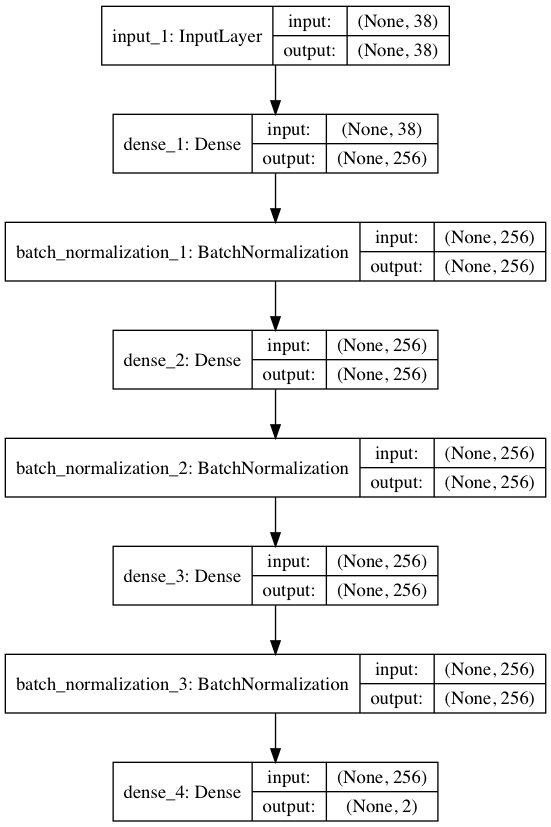
\includegraphics[width=0.5\textwidth,keepaspectratio]{model.png}
	\caption{A model of the \gls{dnn} used in the analysis. }
	\label{fig::nnmodel}
\end{figure}
The model has used Adam optimizer with learning step $0.001$ and batch size of $4000$ data points. Twenty percent of events were used for validation. The two target values were Cartesian components of the truth \gls{hr} vector.

\subsection{Kinematic distributions} 
The results presented here demonstrate the regression plots obtained with the trained DNN. They include the plots from the test sample of $W^+\rightarrow\mu\nu$ at 13 TeV, as well as plots from.  


\section{Technical details}
